%Usar \chapter*{Título do Capítulo} faz com que o capítulo não seja numerado
\chapter{Conclusão} \label{conclusao}

Este trabalho apresentou o projeto do computador de bordo (OBC) para a futura missão do projeto Lodestar da Universidade de Brasília (UnB).

Inicialmente foi realizada uma breve contextualização do tema, seguida de um levantamento dos objetivos do trabalho, onde foram descritos os requisitos exigidos no desenvolvimento e construção do hardware. 

Em seguida, foi apresentada uma revisão teórica onde abordou-se os principais conceitos para o entendimento do design, partindo dos conceitos de nanossatélite, \textit{CubeSats}, PCB, passando pela especificação PC/104 e, por fim, foi feito um breve levantamento de alguns nanossatélites lançados em missões anteriores e que serviram de aprendizado para esse trabalho.

Logo em seguida, iniciou-se o capítulo de desenvolvimento, mostrando ... TO BE CONTINUED


% Colocar diagrama de Gantt

\noindent
\begin{minipage}{\linewidth}
\makebox[\linewidth]{
    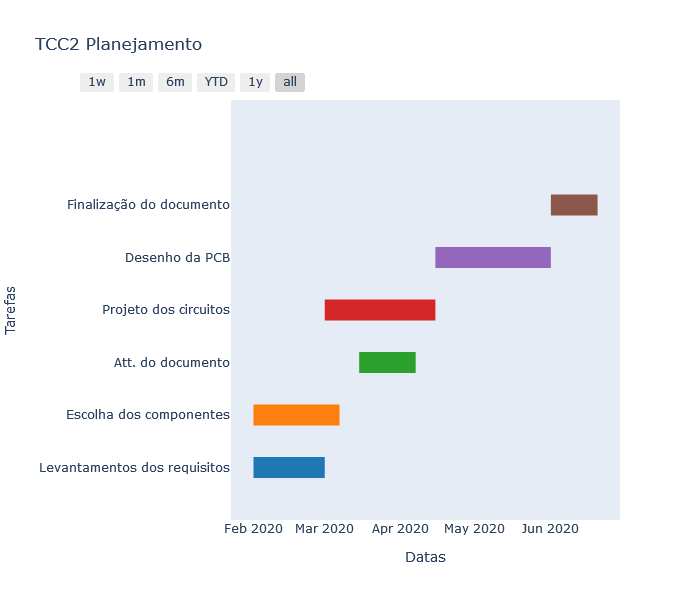
\includegraphics[keepaspectratio=true, scale=0.7]{imagens/TCC2.png}}
\captionof{figure}{Diagrama de Gantt para o TCC2}
\label{tcc2_gantt_fig}
\end{minipage}